\documentclass[tikz, border=10pt]{standalone}
\begin{document}
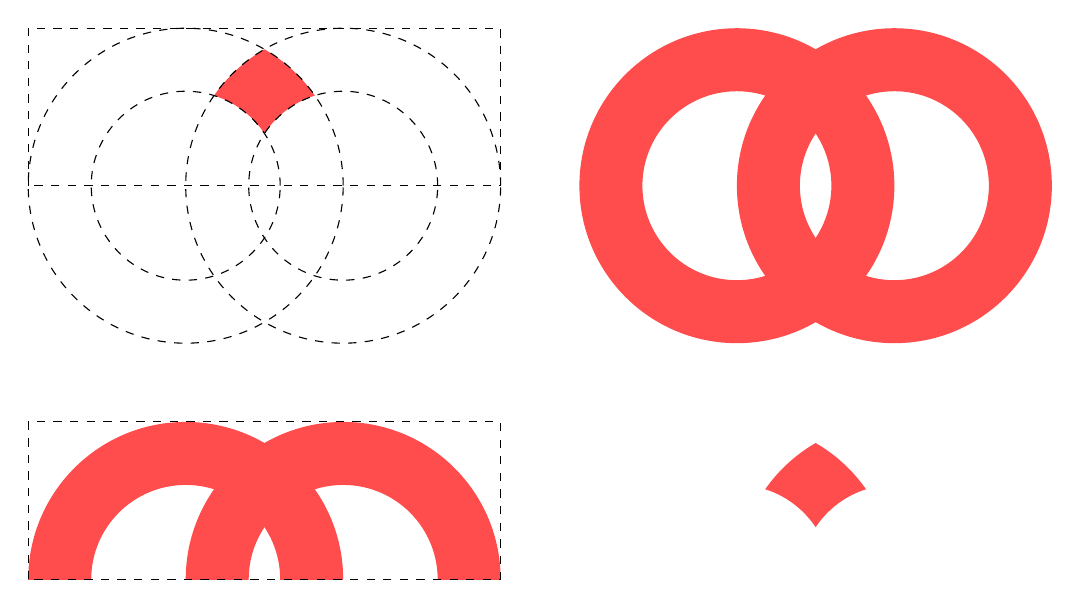
\begin{tikzpicture}[even odd rule]
    \begin{scope}
        \clip (-3, 0) rectangle (3, 2);
        \clip (-1, 0) circle (1.2) (-1, 0) circle (2);
        \fill[red!70] (1, 0) circle (1.2) (1, 0) circle (2);
    \end{scope}
    \draw[dashed] (1, 0) circle (1.2) (1, 0) circle (2);
    \draw[dashed] (-1, 0) circle (1.2) (-1, 0) circle (2);
    \draw[dashed] (-3, 0) rectangle (3, 2);

    \begin{scope}[xshift=7cm]
        \fill[red!70] (1, 0) circle (1.2) (1, 0) circle (2);
        \fill[red!70] (-1, 0) circle (1.2) (-1, 0) circle (2);
    \end{scope}

    \begin{scope}[yshift=-5cm]
        \begin{scope}
            \clip (-3, 0) rectangle (3, 2);
            \fill[red!70] (1, 0) circle (1.2) (1, 0) circle (2);
            \fill[red!70] (-1, 0) circle (1.2) (-1, 0) circle (2);
        \end{scope}
        \draw[dashed] (-3, 0) rectangle (3, 2);
    \end{scope}

    \begin{scope}[xshift=7cm, yshift=-5cm]
        \begin{scope}
            \clip (-3, 0) rectangle (3, 2);
            \clip (-1, 0) circle (1.2) (-1, 0) circle (2);
            \fill[red!70] (1, 0) circle (1.2) (1, 0) circle (2);
        \end{scope}
    \end{scope}

\end{tikzpicture}
\end{document}